%!TEX root = ../TTT4150-Summary.tex
\section{Coordinate frames}

%%%%%%%%%%%%%%%%%%%%%%%%%%%%%%%%%%%%%%%%%%%%%%%%%%%%%%%%%%%%
\subsection{Reference frames}

\subsubsection{Notation}
\begin{itemize}
    \item $\V{v}^n$---velocity given in frame $n$
    \item $\M{R}_p^n$---rotation from frame $p$ to $n$
    \item $\V{\omega}_{ip}^p$---angular rate of frame $p$ w.r.t. $i$, represented in $p$.
\end{itemize}

\subsubsection{Inertial frames and the ECI frame $\{i\}$}
A frame in which Newton's laws of motion apply, i.e. it does not accelerate. All inertial sensors measure relative to an inertial frame. \emph{Earth-centered intertial} (ECI) is an example of this, with origin at the Earth center, not rotating with the earth. (But as the Earth rotates around the sun, ECI is not exactly inertial.)

\subsubsection{ECEF frame $\{e\}$}
Earth-centered, earth-fixed. Rotates relative to ECI with $\omega_{ie} \approx \SI{7.292e-5}{\radian\per\second}$.

\subsubsection{Geographic frame $\{g\}$}
Origin equal to platform origin projected onto the reference ellipsoid. $z$-axis down, normal to ellipsoid surface. $x$-axis north, $y$-axis east. Not inertial.

\subsubsection{Geocentric frame}
Similar to the geographic frame, but $z$-axis down toward Earth center. Also not inertial.

\subsubsection{Tangent plane}
North, east, down as used in daily life. Origin at a fixed point on Earth. Coincides with the geographic frame when the system origin coincides with the tangent frame origin.

\subsubsection{Body frame $\{b\}$}
Attached to the vehicle of interest, often origin at center of gravity. $x$-axis forward, $z$-axis down, and $y$-axis completes the right-handed orthogonal coordinate system (i.e. to the right).

\subsubsection{Platform frame}
Frame centered somewhere on the sensor platform. Usually non-moving wrt. the body frame, so $\M{R}_p^b$ is constant.

\subsubsection{Instrument frame}
The frame along which an instrument measures. (An IMU measures acceleration along the instrument axes, and rotation rate around the instrument frame axes.)

%%%%%%%%%%%%%%%%%%%%%%%%%%%%%%%%%%%%%%%%%%%%%%%%%%%%%%%%%%%%
\subsection{Ellipsoids}

\begin{figure}[htbp]
    \centering
    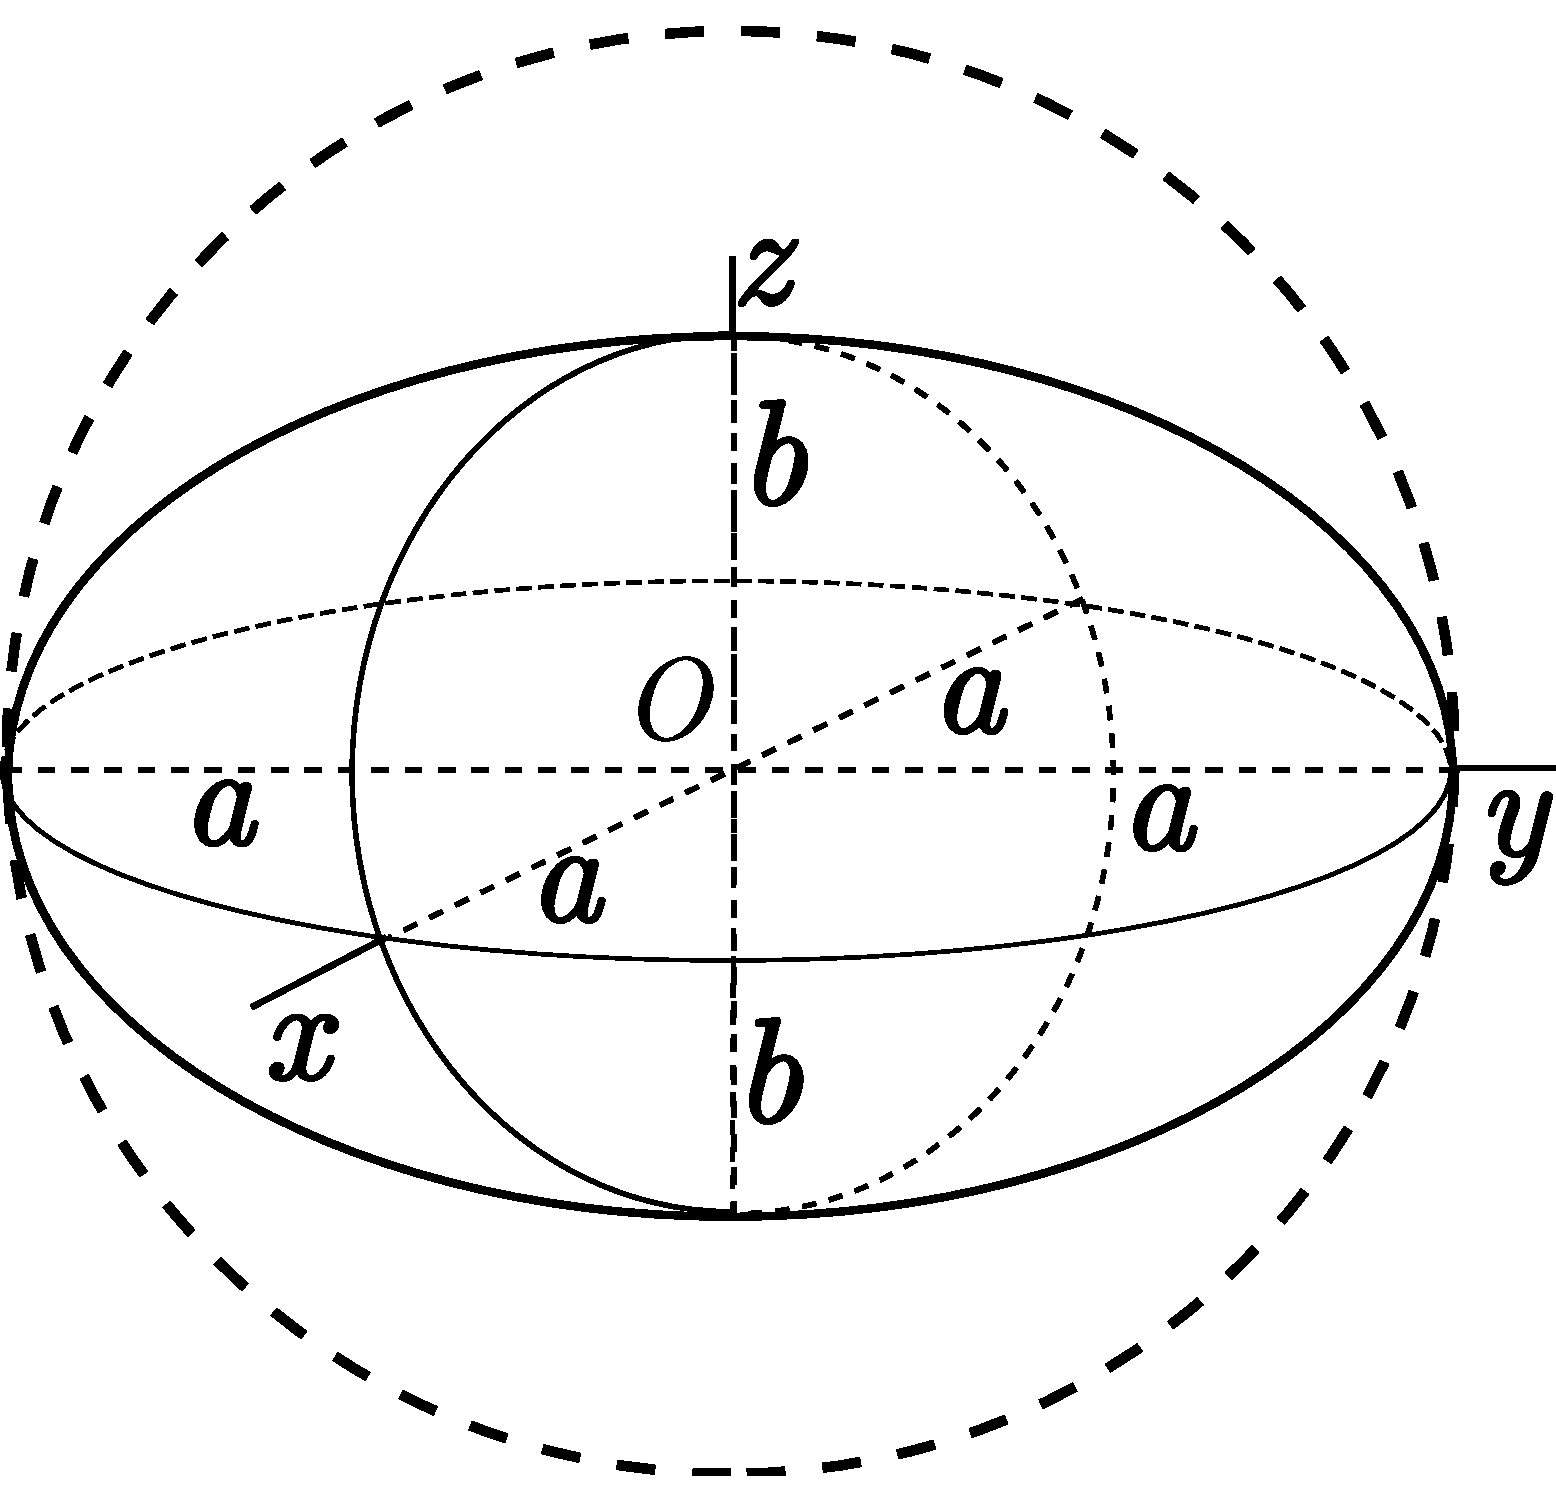
\includegraphics[width=.6\linewidth]{img/ellipsoid}
    \caption{An oblate ellipsoid}
    \label{fig:ellipsoid}
\end{figure}
An ellipsoid is defined by its semi-major axis $a$ and semi-minor axis $b$ (see Figure \ref{fig:ellipsoid}). Its \emph{eccentricity} $e$ is defined by
\begin{equation}
    e^2 = \frac{a^2 - b^2}{a^2} .
\end{equation}
and its flattening $f$ is
\begin{equation}
    f = \frac{a-b}{a} .
\end{equation}

\subsubsection{Radii of curvature}
$M$ is the radius of curvature of a meridian at a given geodetic latitude $\phi$. $N$ is the radius of curvature normal to the meridian at a given $\phi$. Because the Earth is oblate, $M$ is largest at the poles, and smallest at the equator. At the poles, $N = M$, because the radius is the same in all directions.

%%%%%%%%%%%%%%%%%%%%%%%%%%%%%%%%%%%%%%%%%%%%%%%%%%%%%%%%%%%%
\subsection{Geodetic coordinates}

Defined by
\begin{itemize}
    \item latitide $\phi$,
    \item longitude $\lambda$, and
    \item height $h$ above the ellipsoid.
\end{itemize}

%%%%%%%%%%%%%%%%%%%%%%%%%%%%%%%%%%%%%%%%%%%%%%%%%%%%%%%%%%%%
\subsubsection{Definitions of height}

Three surface models are used: The ellipsoid surface, the geoid surface, and the true surface of the earth. The \emph{geoid} is based on what the mean sea level would be based on local gravitation and the earth rotation.

\begin{itemize}
    \item Orthometric height: Height above the geoid.
    \item Geoid height: Height of the geoid above/below the ellipsoid.
    \item Ellipsoidal height: Height above the ellipsoid, measured normal to the surface. This is what GPS uses.
\end{itemize}

%%%%%%%%%%%%%%%%%%%%%%%%%%%%%%%%%%%%%%%%%%%%%%%%%%%%%%%%%%%%
\subsection{Earth-Centered, Earth-Fixed (ECEF) coordinates}

Defined by Cartesian coordinates $X$, $Y$, and $Z$, along the axes in Figure \ref{fig:ellipsoid}. The positive $x$-axis intersects the surface at $\phi = \lambda = 0^\circ$. (The frame is fixed to Earth and rotates with it.)

%%%%%%%%%%%%%%%%%%%%%%%%%%%%%%%%%%%%%%%%%%%%%%%%%%%%%%%%%%%%
\subsection{Conversion from geodetic to ECEF}

For a sphere of radius $R$ we have
\begin{equation}
\begin{split}
    X &= (R+h) \cos \phi \cos \lambda \\
    Y &= (R+h) \cos \phi \sin \lambda \\
    Z &= (R+h) \sin \phi .
\end{split}
\end{equation}

For an ellipsoid with semi-minor axis $a$ and semi-major axis $b$, we have
\begin{equation}
\begin{split}
    X &= (N + h) \cos \phi \cos \lambda \\
    Y &= (N + h) \cos \phi \sin \lambda \\
    Z &= \left( N[1-e^2] + h \right) \sin \phi
\end{split}
\end{equation}
where the \emph{normal radius of curvature} is
\begin{equation}
    N = \frac{a}{\sqrt{1-e^2 \sin^2 \phi}} .
\end{equation}

%%%%%%%%%%%%%%%%%%%%%%%%%%%%%%%%%%%%%%%%%%%%%%%%%%%%%%%%%%%%
\subsection{Conversion from ECEF to geodetic}

Easy for a sphere:
\begin{equation}
\begin{split}
    \phi    &= \atan \frac{Z^2}{\sqrt{X^2 + Y^2}} \\
    \lambda &= \atan \frac{Y}{X}                  \\
    h       &= \sqrt{X^2 + Y^2} \cos \phi + Z \sin \phi - R
\end{split}
\end{equation}

For an ellipse, ECEF to geodetic conversion can be done iteratively or by one of several closed-form solutions.

\subsubsection{Iterative method}
The longitude $\lambda$ is found as
\begin{equation}
    \lambda = \atan \frac{X}{Y} .
\end{equation}

The latitude $\phi$ is found by iterating
\begin{equation}
    \phi_{k+1}
    =
    \atan
    \left(
        \frac{Z}{\rho}
        +
        \frac{N_k e^2 \sin \phi_k}{\rho}
    \right)
\end{equation}
where
\begin{equation}
    \rho = \sqrt{X^2 + Y^2} .
\end{equation}

When $\phi$ is sufficiently accurate, the height $h$ is found by
\begin{equation}
    h = \rho \cos \phi + Z \sin \phi - N(1 - e^2 \sin^2 \phi)
\end{equation}


\subsubsection{Bowring's closed-form method}
Only valid near the Earth surface.
\begin{equation}
\begin{split}
    \phi &= \atan \frac{Z + e^2 b \sin^3 \mu}{\rho - e^2 a \cos^3 \mu} \\
    \mu  &= \atan \frac{Z a}{\rho b}
\end{split}
\end{equation}

\subsubsection{Vermeille's closed-form method}
Closed-form, valid quite far from Earth (including satellite orbits). Really mathy.

%%%%%%%%%%%%%%%%%%%%%%%%%%%%%%%%%%%%%%%%%%%%%%%%%%%%%%%%%%%%
\subsection{Direction cosine matrix}

You have a vector $\V{v}_1$ given in frame $\phi_1$. The unit vectors along the axes of $\phi_1$ are $I_1$, $J_1$, and $K_1$. Similarly, the unit vectors along the axes of $\phi_2$ are $I_2$, $J_2$, and $K_2$.

Then, the direction cosine matrix between the frames is
\begin{equation}
    \M{R}_2^1
    =
    \begin{pmatrix}
        \cos(I_2, I_1) & \cos(I_2, J_1) & \cos(I_2, K_1) \\
        \cos(J_2, I_1) & \cos(J_2, J_1) & \cos(J_2, K_1) \\
        \cos(K_2, I_1) & \cos(K_2, J_1) & \cos(K_2, K_1) \\
    \end{pmatrix}
\end{equation}
